% chktex-file 10
% chktex-file 1
\documentclass{article}
	\def\papertitle{Identifying regime transitions for water governance at a basin scale}
	\def\authors{Shuang Song, Shuai Wang*, Xutong Wu, Yongping Wei, Graeme S. Cumming, Yue Qin, Xilin Wu, Bojie Fu}
	\def\journal{Water Resources Research}
	\def\doi{\#2022WR033819}
% Define title defaults if not defined by user
\providecommand{\lettertitle}{Author Response to Reviews of}
\providecommand{\papertitle}{Title}
\providecommand{\authors}{Authors}
\providecommand{\journal}{Journal}
\providecommand{\doi}{--}

% For using tabularx
\usepackage{tabularx}
\usepackage{booktabs}
\usepackage[includeheadfoot,top=20mm, bottom=20mm, footskip=2.5cm]{geometry}

% Typography
\usepackage[T1]{fontenc}
\usepackage{times}
%\usepackage{mathptmx} % math also in times font
\usepackage{amssymb,amsmath}
\usepackage{microtype}
\usepackage[utf8]{inputenc}

% Misc
\usepackage{graphicx}
\usepackage[hidelinks]{hyperref} %textopdfstring from pandoc
\usepackage{soul} % Highlight using \hl{}

% Table

\usepackage{adjustbox} % center large tables across textwidth by surrounding tabular with \begin{adjustbox}{center}
\renewcommand{\arraystretch}{1.5} % enlarge spacing between rows
\usepackage{caption}
\captionsetup[table]{skip=10pt} % enlarge spacing between caption and table

% Section styles

\usepackage{titlesec}
\titleformat{\section}{\normalfont\large}{\makebox[0pt][r]{\bf \thesection.\hspace{4mm}}}{0em}{\bfseries}
\titleformat{\subsection}{\normalfont}{\makebox[0pt][r]{\bf \thesubsection.\hspace{4mm}}}{0em}{\bfseries}
\titlespacing{\subsection}{0em}{1em}{-0.3em} % left before after

% Paragraph styles

\setlength{\parskip}{0.6\baselineskip}%
\setlength{\parindent}{0pt}%

% Quotation styles


% Quotation styles
\usepackage{framed}
\usepackage{xkeyval} % To define custom key-value pairs

\makeatletter
% Define the keys
\define@key{myquote}{page}{\def\mypage{#1}}
\define@key{myquote}{sline}{\def\mysline{#1}}
\define@key{myquote}{eline}{\def\myeline{#1}}
\presetkeys{myquote}{page=Unknown, sline=Unknown, eline=}{}

\let\oldquote=\quote
\let\endoldquote=\endquote
\renewenvironment{quote}[1][]{%
    \setkeys{myquote}{#1}% Process the keys
    \begin{fquote}
    \ifx\myeline\empty
        \noindent\textbf{Page: \mypage, Line: \mysline} \\
    \else
        \noindent\textbf{Page: \mypage, Line: \mysline\textasciitilde\myeline} \\
    \fi
    \advance\leftmargini -2.4em
    \begin{oldquote}
}{
    \end{oldquote}
    \end{fquote}
}
\makeatother


\usepackage{xcolor}
\newenvironment{fquote}
  {\def\FrameCommand{
	\fboxsep=0.6em % box to text padding
	\fcolorbox{black}{white}}%
	% the "2" can be changed to make the box smaller
    \MakeFramed {\advance\hsize-2\width \FrameRestore}
    \begin{minipage}{\linewidth}
  }
  {\end{minipage}\endMakeFramed}

% Table styles

\let\oldtabular=\tabular
\let\endoldtabular=\endtabular
\renewenvironment{tabular}[1]{\begin{adjustbox}{center}\begin{oldtabular}{#1}}{\end{oldtabular}\end{adjustbox}}


% Shortcuts

%% Let textbf be both, bold and italic
%\DeclareTextFontCommand{\textbf}{\bfseries\em}

%% Add RC and AR to the left of a paragraph
%\def\RC{\makebox[0pt][r]{\bf RC:\hspace{4mm}}}
%\def\AR{\makebox[0pt][r]{AR:\hspace{4mm}}}

%% Define that \RC and \AR should start and format the whole paragraph
\usepackage{suffix}
\long\def\RC#1\par{\makebox[0pt][r]{\bf RC:\hspace{4mm}}\textbf{\textit{#1}}\par} %\RC
\WithSuffix\long\def\RC*#1\par{\textbf{\textit{#1}}\par} %\RC*
\long\def\AR#1\par{\makebox[0pt][r]{AR:\hspace{10pt}}#1\par} %\AR
\WithSuffix\long\def\AR*#1\par{#1\par} %\AR*


%%%
%DIF PREAMBLE EXTENSION ADDED BY LATEXDIFF
%DIF UNDERLINE PREAMBLE %DIF PREAMBLE
\RequirePackage[normalem]{ulem} %DIF PREAMBLE
\RequirePackage{color}\definecolor{RED}{rgb}{1,0,0}\definecolor{BLUE}{rgb}{0,0,1} %DIF PREAMBLE
\providecommand{\DIFadd}[1]{{\protect\color{blue}\uwave{#1}}} %DIF PREAMBLE
\providecommand{\DIFdel}[1]{{\protect\color{red}\sout{#1}}}                      %DIF PREAMBLE
%DIF SAFE PREAMBLE %DIF PREAMBLE
\providecommand{\DIFaddbegin}{} %DIF PREAMBLE
\providecommand{\DIFaddend}{} %DIF PREAMBLE
\providecommand{\DIFdelbegin}{} %DIF PREAMBLE
\providecommand{\DIFdelend}{} %DIF PREAMBLE
%DIF FLOATSAFE PREAMBLE %DIF PREAMBLE
\providecommand{\DIFaddFL}[1]{\DIFadd{#1}} %DIF PREAMBLE
\providecommand{\DIFdelFL}[1]{\DIFdel{#1}} %DIF PREAMBLE
\providecommand{\DIFaddbeginFL}{} %DIF PREAMBLE
\providecommand{\DIFaddendFL}{} %DIF PREAMBLE
\providecommand{\DIFdelbeginFL}{} %DIF PREAMBLE
\providecommand{\DIFdelendFL}{} %DIF PREAMBLE
%DIF END PREAMBLE EXTENSION ADDED BY LATEXDIFF

\usepackage{xr-hyper}
% 参考其它文件的标签 https://texfaq.org/FAQ-extref
\usepackage{xr}
\externaldocument[SI]{../sup/supplementary_information}
\externaldocument[MS]{../main/manuscript}

\begin{document}

% Make title
{\Large\bf \lettertitle}\\[1em]
{\huge \papertitle}\\[1em]
{\authors}\\
{\it \journal, }\texttt{\doi}\\
\hrule

% Legend
\hfill {\bfseries RC:} \textbf{\textit{Reviewer Comment}},\(\quad\) AR\: Author Response, \(\quad\square\) Manuscript text


\graphicspath{{/Users/songshgeo/Documents/VSCode/WGRegimes_YRB_2020/figures/}}

\section{Associate Editor}\label{editor}

\subsection{General comments}
\RC{} Dear Authors, thanks for the submission of the manuscript. We have asked two experts in the relevant fields to review the manuscript. Both reviewers overall find the merit in the manuscript however they also noted several major issues in the current manuscript. With my own reading, I fully agree with the reviewers and would like to highlight a few major issues:

\AR{} Thank you for your constructive comments and for providing us with the opportunity to address the concerns raised by both reviewers. We appreciate the valuable feedback, which has helped us identify areas for improvement in our manuscript. We have carefully considered each point and have made substantial revisions to address these issues. Please find our detailed responses to the highlighted concerns below.

\subsection{Issue \#1}
\RC{} overall the results and discussion are relatively shallow and I would encourage the authors to do deep dive into the results, e.g.\ change points, as also pointed out by both reviewers,

\AR{} We acknowledge the need for a more in-depth analysis of our results. We have re-evaluated our data and expanded the results and discussion sections to include a deeper dive into the findings, specifically regarding the change points mentioned by both reviewers. We have also provided more context and explanation for these changes in the manuscript, which can be found on pages 14\-16 and 18\-21.

\subsection{Issue \#2}
\RC{} I fully agree with Reviewer \#2 that more thorough review of existing and relevant indicators with IWGI,

\AR{} We agree with Reviewer \#2's suggestion to include a more thorough review of existing and relevant indicators with IWGI. We have added a new section in the manuscript discussing these indicators, comparing and contrasting their strengths and weaknesses, and explaining how our approach fills the gaps in the current literature. This new section can be found on pages 5\-7.

\subsection{Issue \#3}
\RC{} I would encourage the authors to look into more recent data (beyond 2013) as pointed out by Reviewer 1. In addition, I find the data in supplementary materials is not accessible, which should be amended. The data access and reproduction of the methodology/results are very important for WRR and our scientific community, so we take the issue related with data accessibility very seriously.

\RC*{} Overall, based on the reviewers' recommendations, I would like to ask the authors to submit a suitably revised manuscript in due course.

\AR{} We appreciate the importance of using up-to-date data in our research. We have now included more recent data in our analysis, extending our dataset up to 2021. The updated data, along with the revised results and discussion, can be found on pages 11-13 and 18-21.

\AR*{} We apologize for the inconvenience caused by the inaccessibility of the supplementary materials. We have rectified this issue by ensuring that all supplementary data and files are now accessible and properly linked within the manuscript. We have also provided a clear description of the data and methodology in the supplementary materials to facilitate reproducibility of our results.

\AR*{} We hope that these revisions address the concerns raised by both reviewers and the associate editor. We are confident that these changes have significantly improved the quality of our manuscript and made it more relevant and valuable to the scientific community. We look forward to your further feedback and the possibility of our manuscript being accepted for publication.


% chktex-file 1
% chktex-file 46
\section{Reviewer \#1}\label{reviewer_1}

\subsection*{Overall comments} % todo

\RC{} This study proposed an integrated index that incorporates water resources, water use, and water allocation to represent the water governance regime in the Yellow River basin. The authors showed an in-depth understanding of the water governance in this basin and made a great effort to represent the status of water governance straightforwardly with the integrated index. The figures were generally well-designed and presented clearly. But I feel the paper lacks details of the results which makes it difficult to understand the paper. Specific comments are listed below.

% 感谢您认可。
% 很抱歉缺少细节,可能会使您难以完全理解我们的研究。
% 为了回应您的担忧,我们已经修改了我们的稿件,并提供了更详细的结果解释。请在下面找到我们对您的具体评论的逐条回复。
\AR{} Thank you for your valuable feedback and for acknowledging our efforts in understanding the water governance in the Yellow River basin. We appreciate your comments regarding the clarity of the figures and our integrated index. Sorry about the lack of details in the results section may have made it difficult to fully comprehend our study. In response to your concerns, we have revised our manuscript and provided a more detailed explanation of the results. Please find our point-by-point response to your specific comments below.

\subsection{Major concern \#1}

% 气候变化在指数中没有明确的体现,这可能是本世纪黄河流量恢复的关键因素。气候变化将是未来该流域面临的巨大挑战。重大的气候变化可能影响流域的适应能力,因此需要不同的治理策略。
\RC{} Climate change is not explicitly represented in the index, which might play a key role in the streamflow recovery in the Yellow River in this century. Climate change would be a great challenge in the basin in the future. Significant climate change may affect the adaptive capacity of a basin and thus require different governance strategies.

% 气候变化的确会产生很多影响,例如改变降水量和蒸发量。但这些影响都会以影响可用水量的形式体现在IWGI之中。
% 在新增加的图表中,我增加了天然水量的图表展示这种变化
% 例如气候变化让可用水量发生改变(scarcity),极端气候让我们难以有效的分配水资源(allocation),对气候变化的适应可能导致社会变革,让人们对愈发侧重于工业和经济发展的治理策略进行反思(priority)。
% 我们现在在讨论中涉及了这些话题。
\AR{} Thanks for the comment that we lacked a discussion of climate change, which has a multitude of impacts e.g., on precipitation and evaporation.
However, these effects are inherently captured within the Integrated Water Governance Index (IWGI) because the available water resources are affected by climate change as consequences.
For clarity, we first modified our expression of SFV-index, which is the indicator highly related to climate change (both in water yield and its fluctuation):

\begin{quote}[page=3, sline=83, eline=88]
	\DIFadd{An important reason for developing this new index is practices of water governance changes throughout development under a hybrid of social and natural drivers.
	First, besides climate change impacts embedded in current water yield concerns, water stress is also tightly related to an }\DIFaddend increasingly insatiable demands from economic activities\DIFdelbegin \DIFdel{such as irrigation and industry; water storage can resolve some but not all of these issues
	}\DIFdelend \DIFaddbegin \DIFadd{, while developing water storage to release the stress~}\DIFaddend~\cite{qin2019,wada2014,huang2021}.
\end{quote}

\begin{quote}
	% TODO page and line numbers
	This indicator integrates the share of runoff being consumed, the share of consumption in these inflexible categories and the historical variability of runoff weighted by storage capacity~\cite{qin2019}, where impacts from both management measures and climate changes are included. The SFV-index, which has many applications, is the most comprehensive index of water stress we know.
\end{quote}

\AR*{} In addition, we added a new graph (Figure~\ref{fig:runoff}~a) in the revised version of supplementary material to demonstrate the changes in runoff. Trend of natural runoff can also be inferred from the measured runoff (Figure~\ref{fig:runoff} from b to d) and water use (Figure~\ref{fig:runoff} from e to g). We quote this figure when discussing climate context, now:

\begin{quote}
	% 一个基本背景是,在用水量总体保持稳定的情况下,黄河流域的径流量已显著低于从前,这是该时期水资源压力重新上升的重要原因。
	Partially because of changed climate~\cite{han2023,liu2020c}, the runoff of the YRB was significantly lower than before when the overall water uses remained stable, which was an important reason for the rise of water stress in this stage (Figure~\ref{fig:runoff} and Figure~\ref{fig:scarcity}).
\end{quote}

\AR*{} Finally, we further discussed the challenges brought by climate changes in the discussion section:

% 我们强调流域治理需要考虑这些因素,但我们可能很难穷尽优秀的流域治理策略需要考虑哪些因素。因此,IWGI至少让我们可以知道在诸多治理因素的共同影响下,流域的未来正在走向何方。
\begin{quote}
	Future's tightly intertwined socio-hydro interactions can lead water governance challenges even more complex and comprehensive, combining resources issues and structural barriers~\cite{huggins2022a}.
	For example, climate change may alter water scarcity levels and make it more difficult to effectively use water due to extreme climate events, strengthening water stress and threatening infrastructures~\cite{liu2017, dibaldassarre2019}.
	Additionally, adapting to climate change could lead to transformations~\cite{sachs2019,barnes2020}, prompting a reevaluation of governance strategies of social water usage (priority and allocation) which is being increasingly altered by current regime transitions.
	It may be difficult to exhaust what is considered in a good watershed governance strategy, but the IWGI at least gives us a sense of where the a river basin is heading and how challenged.
\end{quote}

\subsection{Major concern \#2}
% 结果是总结性的。我建议提供更多关于三个指数和IWGI结果的信息。例如,三个指标的结果,以及分区域的结果。请解释IS、IP、IA和IWGI这三个指标的范围,以及不同数值的含义。这些细节可以帮助读者理解结果的合理性。
\RC{} The results are summative. I would suggest providing more information on the results of the three indices and the IWGI.\ For example, the results of the three indices, and the results for the sub-regions. And please explain the range of the three indicators, IS, IP, IA, and the IWGI, and the meanings of different values. These details could help readers understand the reasonability of the results.

% 感谢您指出这一点,非常抱歉过于总结性的手稿带来的困惑。
% 在新的手稿中,我们将各指数的情况总结到补充材料,并在正文中对有关各指数情况的图表总结。
% 在方法中,我们补充了指标的取值范围(三个子指标的变化范围都是0~1)。
\AR{} Thank you for pointing this out, and we apologize for the confusion caused by the overly conclusive manuscript. In the revised manuscript, we have summarized the indicators by graphs with description in supplementary material:in the supplementary material.

% TODO 这里记得写一下是哪几个附图
\AR*{} Figure SX to SX are three indicators changing trends with different regions' contribution.

\begin{quote}
	The index of stress (SFV indicator, IS) in the study period (including three different periods) showed a change trend of first decreasing, then rapidly increasing, and finally slightly decreasing again (Figure~\ref{fig:scarcity}~A), indicating that water resource pressure first decreased, then rapidly increased, and then stabilized.
	Among the four different regions (Figure~\ref{fig:scarcity}~B), the source region (SR) has almost no contribution to IS changes in the three periods, and the downstream region (DR) only has a weak negative contribution in the governance transforming regime and the adaptation oriented regime.
	The upper and middle reaches (UR and MR) had the greatest impact on the IS changes. Wherein, the upper region (UR) made the greatest contribution during the massive supply regime and governance transforming regime, while the middle reaches made the greatest contribution in adaptation oriented regime.

	In terms of water use purpose indicator, IP remained basically unchanged in a massive supply regime, but showed a rapid decline in the period of governance transformation and adaptation oriented regime (Figure~\ref{fig:priority}~A).
	Throughout the three periods, the change of irrigation water dominated the change of the IP, while urban and rural water for human settlements and rural livestock had almost no influence on the change of IP (Figure~\ref{fig:allocation}~B).

	The water allocation (IA) showed an obvious ``V-shaped'' trend, indicating that water resources in the different regions within the YRB first gradually moved away from uniform distribution, and then gradually tended to uniform distribution since 2000 (Figure~\ref{fig:allocation}).
\end{quote}

\AR*{} In addition, ranges of three indicators and meaning of their values are further explained in the methodology section, now:

\begin{quote}
	where $I'_x$ is calculated by Min-Max normalization of $I_x$ (thus ranges from zero to one):
	\begin{equation}
		I'_x = (I_x - I_{x, \min}) / (I_{x, \max} - I_{x, \min})
	\end{equation}
\end{quote}

\subsection{Major concern \#3}
% 本研究中使用的数据似乎有不同的时间段,大多数数据来自2013年之前。近十年来,黄河的水文状况和水治理应该发生了重大变化。因此,结合近十年的结果将使这项研究更加可靠。
\RC{} The data used in this study seem to have different time periods, and most data are from before 2013. The hydrological regime and water governance in the Yellow River should have changed significantly in the recent decade. Therefore, incorporating the result from the recent decade would make this study more solid.

% 感谢审稿人的宝贵建议,但出于以下原因,我们无法在新的手稿中将研究时段后延至今
\AR{} Thanks for the reviewer's valuable advice, but for the following reasons, we are unable to postpone the study period to date in the main text. Instead, we added robustness test by using different-source data in supplementary material.

% 首先,本研究结论希望展现黄河水治理演变过程,尤其是重点关注1978到2001年之间的治理转型过程。尽管许多数据能在近二十年间计算IWGI,但代价是忽略了更远的时间段。而正如我们在新手稿的方法部分所补充说明的,使用不同的数据源容易造成时间不连续的问题(通常它们的统计口径是不一样的)。
\AR*{} Firstly, the conclusion of this study aims to show the evolution process of water governance of the Yellow River, especially focusing on the governance transformation between 1978 and 2001. Although many dataset allow IWGI to be calculated over the last two decades, the cost is to ignore the more important past periods. In addition, it's difficult to assimilate the different data sources because datasets usually have different statistical approach when categorizing water use sectors. Now, we added an explanation in the methods section of the new manuscript:

\begin{quote}
	Since the IWGI essentially comprises by three aspects' indicator with same weights, its prerequisite is to keep the same data source for each indicator throughout time, to ensure time series continuity.
\end{quote}

\AR*{} Secondly, as the reviewer noticed, we used multiple-source dataset to implement our approach, which means time periods of a coherent analysis is limited by the shortest data. To cover study period from 1960s to 2000s, water use data developed by \citeA{zhou2020} is the most good quality and widely used dataset. The shortage, however, is not enough to cover the period after 2013. We contacted the original author team, but only confirmed that latest dataset is still unavailable. As some of the source data used to produce this crucial dataset could not be easily supplemented, this was not an effort that could be supplemented in this study. Therefore, we decided to keep the analysis discontinued in 2013 in main texts:

\begin{quote}
	Another limitation is the lack of latest datasets which is coherent with the historical datasets, so our analysis had to discontinued in 2013 despite potential shifts existing.
\end{quote}

\AR*{} Last, we tried our best to strengthen robustness of this study despite the above limitations. We calculated IWGI by using another data source for the past two decades. Since our results suggest no significant regime change, we think it is robust that the YRB experienced two significant water governance regime changes.

\begin{quote}
	As a supplement, we examined IWGI framework with fewer datasets from different source in recent decades where showing no significant regime changes (supplementary Figure~\ref{fig:summary}).  % TODO 补充材料新图
\end{quote}

\subsection{Major concern \#4}
% 这三个指标之间可能存在相互作用/相互联系。作者是否检查了指标之间的关系?
\RC{} There might be interactions/interconnections among the three indicators. Did the authors examine the relations between the indicators?

\AR{} Yes, we did examination for the interconnections between the three indicators. Sorry we didn't make the information accessible. Now, we added a table to describe this in the supplementary material (Table~\ref{tab:corr}).

% Table generated by Excel2LaTeX from sheet '相关性情况'
\begin{table}[htbp]
    \centering
    \caption{The correlation of the Integrated Governance Index (IWGI) and its three sub-indicators (IS, IP, IA)}
      \begin{tabularx}{\textwidth}{XXXXXXX}
      \toprule
      Period & \multicolumn{1}{l}{IS vs IP} & \multicolumn{1}{l}{IS vs IA} & IP vs IA & \multicolumn{1}{l}{IP vs IWGI} & \multicolumn{1}{l}{IA vs IWGI} & \multicolumn{1}{l}{IS vs IWGI} \\
      \midrule
      P1 to P3 & \multicolumn{1}{l}{-0.75 *} & -0.29 & 0.36 & 0.37  & \multicolumn{1}{l}{0.75 *} & 0.14 \\
      P1    & -0.08 & -0.31 & 0.06 & 0.14  & 0.51  & 0.65 \\
      P2    & \multicolumn{1}{l}{-0.90 *} & \multicolumn{1}{l}{-0.87 *} & 0.77 * & -0.18 & -0.13 & 0.5 \\
      P3    & 0     & -0.38 & -0.86 * & -0.33 & 0.61  & 0 \\
      \bottomrule
      \end{tabularx}%
    \label{tab:corr}%
\end{table}%


\begin{quote}
	By analyzing the correlation of the integrated management index (IWGI) and its three sub-indexes: stress (IS), priority (IP) and allocation (IA) in three different periods, namely, the massive supply regime (P1: $1965 \sim 1978$), governance transforming regime (P2: $1979 \sim 2001$) and adaptation oriented regime (P3: $2002 \sim 2013$), the following results are obtained.

	When we focus on the correlation from P1 to P3, the results show significant negative correlation between IS and IP (correlation coefficient is $r = -0.75$, $p < 0.01$), indicating that there is a strong negative relationship between IS and IP.\
	On the other hand, there is a significant positive correlation between IA and IWGI (correlation coefficients are $r = 0.75$, $p < 0.01$), indicating a positive relationship between IA and IWGI.\ However, the correlations of other combinations are not statistically significant overall.

	The correlations between time periods are very different with the overall trend above.
	There is no significant correlation between any indicator combinations in the massive supply regime (P1).
	In the governance transforming regime (P2), there is a significant negative correlation between IS and IP (correlation coefficient $r = -0.90$, $p < 0.01$), a significant negative correlation between IS and IA (correlation coefficient $r = -0.87$, $p < 0.01$), and a significant positive correlation between IP and IA (correlation coefficient $r = 0.77$, $p < 0.01$).
	The correlations between IS and IP, IS and IA, and IS and IWGI were not statistically significant in the adaptation oriented regime (P3). However, there is a significant negative correlation between IP and IA (correlation coefficients are $r = -0.86$, $p < 0.01$).
\end{quote}

\AR*{} In addition, note that strictly independent of indicators is not required in our approach, as three aspects are intertwined in essence (we explained this in the introduction).
% 这是因为,如果两个子指标在某时期内相关性显著,可能说明两者在该时期同时受到某些治理驱动因素的共同作用,这是可能发生的。
This is because a significant correlation between two indicators in a given period may indicate that both were simultaneously affected by some governance drivers during that period, which is possible.
% 但同样,若两个指标始终都存在较强的关联,则可能说明稳态转换并不显著,IWGI同时考虑三者的意义也存疑。
Similarly, if there is always a strong correlation between the two indicators, it may indicate that the steady-state transformation is not significant, and the significance of IWGI considering the three indicators at the same time is doubtful.
% 然而,正如我们在表x中所展示的,IS, IP, IA三者两两之间的关系在不同稳态下都有不同的特征,这佐证了我们IWGI同时考虑三者的意义,以及稳态转换的存在。
However, as we have shown in Table~\ref{tab:corr}, the relationship between IS, IP and IA has different characteristics under different regimes, which proves that IWGI considers the significance of the three aspects at the same time, as well as the existence of regime shifts.

\subsection{Major concern \#5}
% IWGI在“应力”方面包含储层存储信息。输水能力是衡量水治理/水社会复原力的重要指标。
\RC{} The IWGI includes reservoir storage information in the ``stress'' aspect. However, the water conveyance ability is not represented, which is also an important indicator of water governance/hydrosocial resilience.

% 短期的输水能力是衡量水治理/水社会复原力的重要指标
% 但年尺度上,变化不大
\AR{} We agree that conveyance is crucial to water governance/water society resilience, especially in the short term. However, the IWGI in this study focuses on annual time resolution. At this scale, conveyance has a less significant impact on water governance. From this point of view, there are two reasons that IWGI doesn't have to consider this in our study:

% 输水是水治理的手段,我们更侧重于这种治理的结果。
\AR*{} Firstly, water conveyance is more like an approach of water governance, and we focus more on the outcomes -i.e., how water stress is relieved by conveyance; how it help provision to specific sectors with higher priority; how convert water changes allocation of water resources \dots

% 水治理很复杂,考虑到越来越多的要素会增加其复杂度。Scarcity是本研究使用最复杂的指标,因为这是一个经过检验的,可以有效表征的指数。如果经过检验影响不大,没有必要增加复杂度。
\AR*{} Secondly, water governance is comprehensive, and taking into account more and more elements increases its complexity. SFV-index is the most complex index used in this study, because it is a tested index that can be effectively represented. If not necessary, we prefer not to include more complexity.

% 我们检验过了年尺度的输水数据,基本变化不大
\AR*{} Finally, since we agree the conveyance is a good view to investigate water governance, we added an examination of the monthly conveyance flow differences of the major reservoirs and their variability in supplementary material. According to the Yellow River Water Conservancy Commission (YRCC, data source), these reservoirs are mainly for managing and regulating the whole basin. The result (Figure~\ref{fig:conveyance}) shows that variability increased in the later regimes, supporting our main results that regulation plays a more significant role since the governance transforming regime (P2). We also appropriately modified the description in main text:

\begin{quote}
	Ensuing the P2, the number of new reservoirs decreased but boosted their role in water regulating and management (more red circles in Figure~\ref{fig:Causes}~C, and larger water conveyance variability in Supplementary Materials Figure~S7).  % todo 检查图引用
\end{quote}

\subsection{Major concern \#6}
% 我建议在标题中加上“黄河流域”。因为没有对IWGI的适用性和有效性进行测试或讨论。它能在其他盆地使用吗?使用索引的先决条件是什么?
\RC{} I would suggest adding ``Yellow River basin'' in the title. Because the applicability and validity of the IWGI were not tested or discussed. Can it be used in other basins? What is the prerequisite for using the index?

% 感谢你的提议,我们现在在标题中增加了黄河流域,新的标题是:
\AR{} Thanks to your proposal, we have now added the Yellow River Basin to the title, and the new title is: \textbf{``Identifying regime transitions for water governance: Take the Yellow River Basin in China as case''}

% 关于IWGI的泛用性,实际上我们曾在讨论中讨论了这一点。
% 非常抱歉先前的讨论似乎不够明确,我们在修改后的论文中重新澄清了这点。
\AR*{} Regarding the generality of IWGI, we actually discussed this in our discussion. I am very sorry that the previous discussion seems not clear enough, and we have clarified this point again in the revised manuscript.

\begin{quote}
	One of the main limitations in the approach is the lack of multi-sources data in long-term period worldwide, which means there is still a gap between comprehensively identifying and applying the IWGI widely.
	We propose that all water governance issues, however, can change ``who gets water, when and how'' so monitoring such an integrated index is essential, even use simpler indicators.
	We suggest that choices of indicators for different aspects can be adapted according to available datasets -e.g., replace the SFV-index (IA) with simpler scarcity index or proportion-based priority indicator (IP) by complicated one.
\end{quote}

% 此外,我们如今在方法部分提到了使用它的先决条件,使用同样数据源保证单一子指标的时间序列连贯性,而不同子指标可以采用不同的数据源。
\AR*{} In addition, we have now mentioned in the methods section:

\begin{quote}
	Since the IWGI essentially comprises by three aspects' indicator with same weights, its prerequisite is to keep the same data source for each indicator throughout time, to ensure time series continuity.
	However, vary data sources can be used when estimating the specific indicator or cross different indicators, which makes IWGI a flexible framework for substituted indicators.
\end{quote}

\subsection{Major concern \#7}
% 最好在引言部分解释“水治理机制”的概念,然后解释使用综合指数IWGI代表水治理机制的必要性。
\RC{} It would be better to explain the concept ``water governance regime'' in Introduction and then explain the necessity of using the integrated index IWGI for representing the water governance regime.

% 感谢你的建议,我们在引言部分为“水治理机制”提供了一个简短但明确的解释:
\AR{} Thanks for your advice, we nor provide a short but clear explanation of the ``water governance regime'' in the introduction:

\begin{quote}
	A critical step in understanding the successes and failures of water governance is to identify the different regimes that underpin it~\cite{kjellen2015, grafton2013}.
	Regimes of water governance, the general guidelines of practices, arise within linked human-water systems (based on management, institutions, and exploitation) to create local equilibria in social-ecological structures and functions~\cite{falkenmark2021,bressers2013,loch2020,pahl-wostl2007}.
\end{quote}

% 我们还为这种指数的必要性做出了补充:
\AR*{} We also add to the argument for the need for such an index:

\begin{quote}
	Standing from water side for comprehensively quantify governance outcomes, here we aim to develop an integrated water governance index to identify its changes by involving apportions of water uses between regions and sectors.

	An important reason for developing this new index is practices of water governance changes throughout development under a hybrid of social and natural drivers.
\end{quote}

\subsection{Detailed issues}

% 我没有在引用的文献中找到“用水的三个核心方面”。这三个方面是作者提出的吗?
\RC{} Line 57\-62: I did not find the ``three core aspects of water use'' in the cited reference. Were the three aspects put forward by the authors?

\RC{} Line 92: missing information for the citation?

\RC{} Line 94\-95: the sentence is unclear.

\RC{} Line 121: Repeated citation Qin et al. 2019.

\RC{} Line 122: It would be better to introduce the calculation of SFV in the main text.

\RC{} Equation (6): Why is the numerator WUpro not WUnon-pro? Please check the equation.

\RC{} Equation (7): CEM => AEM?\

\RC{} Line 154: Please explain the source of irrigated area data.

\RC{} Fig.2A, p<0.01 or p<0.001? (line 147 says that α=0.001 was used for the change-point detection).

\RC{} Fig.2C: How were the directions determined?

\RC{} Fig.3C: What do the dashed lines denote?

\RC{} Line 187: what is "social transformation"?

\RC{} Line 208: the IWGI was proposed in this study, here the citations of Loch's and Turton's studies are not appropriate.

\RC{} Line 273: adapted => adopted?

\RC{} Line 275: biophysical? Please check the sentence.

\AR{} \dots


\section{Reviewer \#2}\label{reviewer_2}

\subsection*{Reviewer \#2 Evaluations:}

\begin{itemize}
    \item Recommendation (Required): Return to author for minor revisions
    \item Significant: The paper has some unclear or incomplete reasoning but will likely be a significant contribution with revision and clarification.
    \item Supported: Yes
    \item Referencing: Yes
    \item Quality: Yes, it is well-written, logically organized, and the figures and tables are appropriate.
    \item Data: Yes
    \item Accurate Key Points: Yes
\end{itemize}

\subsection*{General comments}

\RC{} Thank you for sharing your revised manuscript. The revised manuscript was very carefully constructed. This revision solved most of my questions, but there were some incomplete and vague parts in the response to ``2.7. Comment \#7''.

\RC*{} I agree that the change of the system is still a result of the accumulation of water governance practices in period. However, it was clear from your results and discussion that these system changes are dictated by specific factors (historical events): e.g., the Chinese slogan ``human will conquer nature'', rapid expansion of irrigated farmland and water diversion facilities so on, in the P1. I suggest that you organize them in a table that shows those factors (historical events) that are causing the ``emergence'' of each complex system. (Figure 4 is too conceptual for the historical phenomenon you were describing.) I believe that this will make the characteristics of each regime clearer.

\RC{} The ``social atmosphere'' is an interesting term, but very vague. First of all, please define what it is (I have never heard of such a term in previous studies in my field). At the very least, you should discuss what ``social atmosphere'' is in the Discussion. Furthermore, I really wonder how your research and the proposed index can be practically contribute to understanding ``the successes and failures of water governanceis'' created by the ``social atmosphere''. Perhaps this ``social atmosphere'' is the most troubling and important factor to understand in water governance regime.

\AR{} Thank you for raising an intriguing point of discussion on the concept of ``social atmosphere''. We have taken your feedback into account and provided a definition in the revised manuscript to elucidate this term:

\begin{quote}[page=footnotes from Figure~3 and Table~1]
    Here, social atmosphere refers to the sociocultural context in which people live or in which something happens, including the culture that the individual was educated or lives.
\end{quote}

\AR*{} We maintain a cautious stance regarding the assertion that changes in the ``social atmosphere'' directly lead to shifts in stable states, as our findings do not establish a causal relationship between the two. Nevertheless, as depicted in the newly added Table~1,

% Table generated by Excel2LaTeX from sheet 'Sheet1'
\begin{table}[htbp]
    \centering
    \caption{Brief summary of regime transitions for water governance at the Yellow River Basin}
      \begin{tabularx}{\textwidth}{p{0.15\textwidth} p{0.15\textwidth} p{0.2\textwidth} p{0.5\textwidth}}
      \toprule
      Time  & Closet social atmosphere$^*$ & Regime & Main trait \\
      \midrule
      $1965-1978$ & 1960s: Conquering nature & massive supply regime & boost water supply for services (mainly provisioning purposes then -livestock and crops) by constructing reservoirs and channels \\
      $1979-2001$ & 1978: reform and opening-up & governance transforming regime & triggered institutional changes for rapid enhancement of overall social adaptive capacity to severe water stresses \\
      $2002-2013$ & 2002: Environmental regulating & adaptation-oriented regime & adapting to stable high water stress with trade-offs between water-dependent regions and sectors \\
      \bottomrule
      \end{tabularx}\label{tab:regimes}%

      \footnotesize
      $^*$ Social atmosphere refers to the sociocultural context in which people live or in which something happens, including the culture that the individual was educated or lives.
  \end{table}%


\AR*{} prompted by your suggestion, a temporal co-occurrence between the two is observable. We discussed it more in the revised manuscript:

\begin{quote}[page=10, sline=265, eline=269]
    These regime shifts, as comprehensive outcomes of complex human-water interactions, are coincidentally well presented by several well-known and dominated social atmospheres (Table~1).
    The social atmospheres refers to the sociocultural context in which people live or in which something happens, underlying the direction of practices of water governance during a regime, despite lack of strict causality evidence.
\end{quote}

\AR*{} The evolution of the ``social atmosphere'' could potentially be a consequence of changes in human-water relations or a catalyst for such transformations. We appreciate your perspective that this shift might represent a breakthrough in addressing complex challenges in future studies. We have enriched our discussion with additional insights to reflect on this complex interplay. However, for the scope of this current study, the evidence at our disposal does not permit an extensive exploration centered on this aspect. It's interesting to delve deeper into this intricate relationship in our future work, backed by comprehensive data and analyses.

\subsection*{Minor comment}

\RC{} I couldn't access the link http://www.yrcc.gov.cn/hhyl/hhjs/ in the Supporting Informations. Please confirm it.

\AR{} Sorry to hear that. However, we double-checked that this link is still accessible. It's a page from the official website of Yellow River Conservancy Commission (YRCC). We also uploaded the dataset ``big\_events.csv'' of the web page is made by using the web crawler in the open-sourced Zenodo repo.


\bibliography{../mybibtex.bib}
\bibliographystyle{apacite}

\appendix
\begin{figure}[!htb]
	\centering
	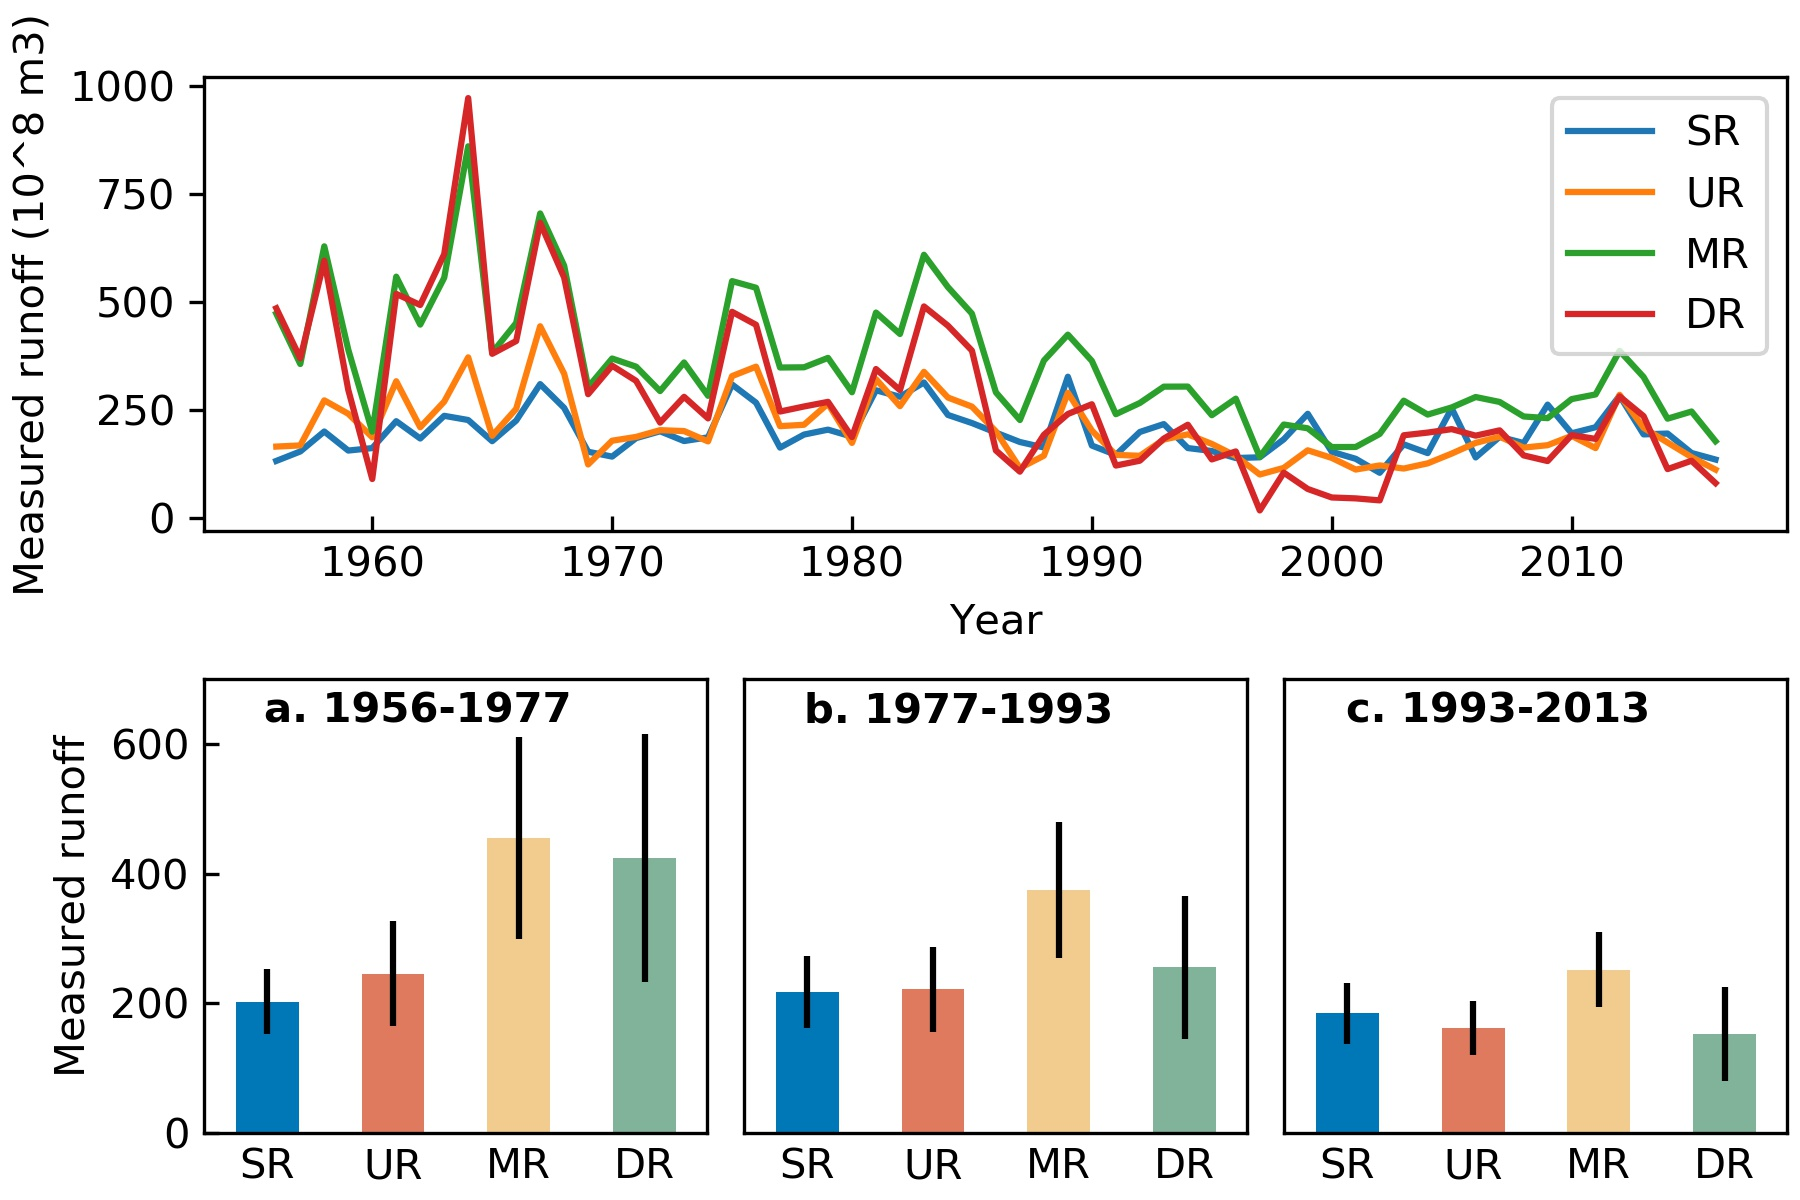
\includegraphics[width=\textwidth]{sup/sf_measured_runoff.jpg}
	\caption{
		\textbf{a.} Measured runoff of different regions in the Yellow River Basin from 1965 to 2013.
		\textbf{b.} Measured runoff of different regions under different water governance regimes.
		\textbf{c.} Natural river runoff of different regions under different water governance regimes.
	}\label{fig:runoff}
\end{figure}


\begin{figure}[htb]
	\centering
	\includegraphics[width=\textwidth]{sup/priority.jpg}
	\caption{Changing trend of the indicator of priority}\label{fig:priority}
\end{figure}

\begin{figure}[htb]
	\centering
	\includegraphics[width=0.7\textwidth]{sup/allocation.png}
	\caption{Changing trend of the indicator of allocation}\label{fig:allocation}
\end{figure}

\begin{figure}[htb]
	\centering
	\includegraphics[width=\textwidth]{sup/scarcity.png}
	\caption{Changing trend of the indicator of stress}\label{fig:scarcity}
\end{figure}


\begin{figure}[htb]
	\centering
	\includegraphics[width=0.8\textwidth]{sup/conveyance.png}
	\caption{Monthly conveyance flow differences of the reservoirs mainly for managing and regulating the whole basin and their variability}\label{fig:conveyance}
\end{figure}

\end{document}
